%Writeup for ENGR202 Lab 3
%If editing in vim/vi please insert your own line breaks! This will help keep the file cleaner and easier to edit.
\documentclass{article}
\usepackage{graphicx}
\graphicspath{ {images/} }
\title{Chapter 3 Lab Writeup}
\author{Zach Thompson et all}
\begin{document}

\maketitle{}

%BEGIN ZACH
\section*{Overview}
\paragraph{}
The purpose of this lab is to evaluate non-ideal components and to simulate them using LTSpice. This is necessary because components in real life
do not have ideal properties and are not perfect. This impacts the circuit and is necessary to understand how to simulate. In this lab we evaluate how the 
given value of a resistor varies from it's measured value as well as how other components vary in measurement from their given values. 


\section*{Process}
\paragraph{}
In order to achieve the purpose of this lab several tools were used. The tools used include an oscilloscope, a function generator, a voltage source, 
a digital multi-meter, and LTSpice. LTSpice was used to simulate the circuits and the rest of the tools were used to measure a physical circuit.

\paragraph{}
Several circuits were analyzed. First a resistor network voltage divider with a DC source was analyzed, then again with an AC source. After that an LR circuit 
was analyzed.

\section*{Results}
\paragraph{}
Here are the results for the various experiments that were conducted in this lab.

\subsection*{Non-Ideal Resistors}
\paragraph{}
For the given circuit an output voltage was found for the voltage divider. The output voltage was found to be 2.5V. Then the given circuit was constructed with 
non-ideal components. For $100\Omega{}$ resistors the resistance tolerance was found to be within $5\Omega{}$ of the given resistance. With the circuit constructed from
non-ideal components the output voltage was found to be 2.498V which was very close to the ideal voltage.

\subsection*{Non-Ideal Voltage Source}
\paragraph{}
For this part of the lab an AC circuit with a resistive load was analyzed. The circuit was setup with two different loads and measured. For both circuits the 
amplitude of the voltage source was measured to be 9V. The voltage was then measured across a $1k$$\Omega{}$ resistor and was found to be 8.4V. The resistor was then 
replaced with a $220\Omega{}$ resistor and the voltage was found to be 7.2V. 

\paragraph{}
Using the recorded values and the given equations several properties of the voltage source could be found. $R_{out}$ was found to be $77.39\Omega{}$. With $R_{out}$ 
we were then able to calculate $X_{out}$ to be $j113.181$. Now the total impedance of the function generator could be found as $77.39 + j113.181\Omega{}$ in 
rectangular form and $137.11\angle{}55.64^\circ{}$ in polar form.

\subsection*{Other Non-Ideal Components}
\paragraph{}
An inductor was inspected next. The resistance of a 10mH inductor was measured with a digital multimeter and the equivalent series resistance was found 
to be $22.17\Omega{}$.
%END ZACH

%BEGIN KYLE
\subsection*{Modeling Non-Ideality in LTSpice}
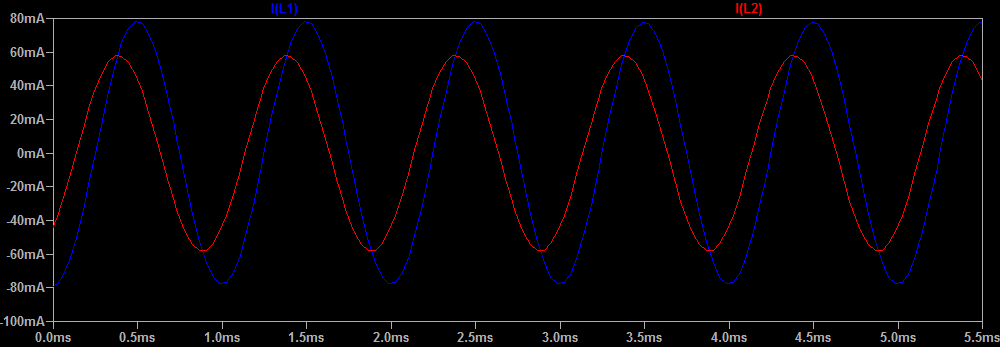
\includegraphics[width=\textwidth]{graph}
%END KYLE

\end{document}
